\documentclass[aspectratio=169]{beamer}
\geometry{paperwidth=160mm,paperheight=100mm}
\usepackage{beamerthemesidebar}
\usepackage{hyperref}
\usepackage{color}
\usepackage{multimedia}
\usepackage{colortbl}
\usepackage{amsmath}
\usepackage{empheq}
\usepackage{cancel}
\usepackage{amssymb}
\usepackage{amsfonts}
\usepackage{lipsum}
\usepackage{tcolorbox}
\usepackage{tabularx}
\usepackage{caption}
\usepackage{bm}

\setbeamersize{sidebar width right=0pt}
\setbeamertemplate{footline}[frame number]
%
\definecolor{orange}{RGB}{250,167,12}
\definecolor{yellow}{RGB}{246,250,12}
\definecolor{green}{RGB}{128,238,1}
\definecolor{black}{RGB}{0,0,0}
\definecolor{blue}{RGB}{0,0,255}
\definecolor{red}{RGB}{255,0,0}
\definecolor{sepia}{RGB}{94,38,18}
\newcommand{\ve}[1]{{\rm\bf {#1}}}
\newcommand{\q}[1]{\textcolor{blue}{#1}}
\newcommand{\blue}[1]{\textcolor{blue}{#1}}
\newcommand{\sepia}[1]{\textcolor{sepia}{#1}}
\newcommand{\red}[1]{\textcolor{red}{#1}}
\newcommand{\green}[1]{\textcolor{green}{#1}}
\newcommand{\yellow}[1]{\textcolor{yellow}{#1}}
\newcommand{\orange}[1]{\textcolor{orange}{#1}}
\definecolor{burlywood}{RGB}{255,211,155}
\definecolor{chocolate}{RGB}{255,127,36}
\definecolor{tan}{RGB}{210,180,140}
%
\def\onethird{{\textstyle{1\over3}}}
\def\twothirds{{\textstyle{2\over3}}}
\def\fourthirds{{\textstyle{4\over3}}}
\def\onehalf{{\textstyle{1\over2}}}
\def\threehalfs{{\textstyle{3\over2}}}
%
\newcommand{\pd}{\partial}
\newcommand{\aMLT}{\alpha_{\rm MLT}}
\newcommand{\Fconv}{F_{\rm conv}}
\newcommand{\Frad}{F_{\rm rad}}
\newcommand{\Hp}{H_p}
\newcommand{\prad}{p_{\rm rad}}
\newcommand{\pgas}{p_{\rm gas}}
%
\title{Theoretical Astrophysics I: Physics of Sun and Stars\\
Lecture 4: Convective energy transport}
\author{\texorpdfstring{\sepia{Petri K\"{a}pyl\"{a} Ivan Mili\'{c}}\newline\blue{\url{pkapyla, milic@leibniz-kis.de}}}{}}
\institute{Institut f\"ur Sonnenphysik - KIS, Freiburg}
\date{\today}
%
\begin{document}
\frame{\titlepage}

\section{Equation of state}
\frame{
	\frametitle{Energy transport mechanisms in stars}
	\begin{itemize}
		\item Radiation: photons transport the energy. Mean
                  free path is very short and this can be modeled as a
                  diffusion process down the temperature gradient, i.e.,
                  \begin{equation}
                    {\bf F}_{\rm rad} = - K_{\rm rad} \bm\nabla T,\label{equ:Frad}
                  \end{equation}
                  where $K_{\rm rad}$ is the radiative conductivity.
		\item Conduction: heat is transported because of
                  collisions of particles. Analogous to
                  \ref{equ:Frad}, this is written as
                  \begin{equation}
                    {\bf F}_{\rm cd} = - K_{\rm cd} \bm\nabla T.\label{equ:Fcond}
                  \end{equation}
                  Typically $K_{\rm rad} \gg K_{\rm cd}$ (\blue{Except
                    where?}).
		\item Convection: gas is opaque to radiation, becomes
                  \emph{unstable}, and fluid motions transport the
                  energy. This leads to very complicated dynamics and
                  cannot in general be represented in equally simple
                  terms as radiation or conduction.
	\end{itemize}
}
%
\frame{
\frametitle{Intuitive picture of convective instability}
\begin{minipage}{0.4\linewidth}
\begin{itemize}
	\item Consider a fluid element with density $\rho_1$ and
          pressure $p_1$ displaced upward to a level where
          $\rho=\rho_2$ and $p=p_2$.
	\item If the density inside the element ($\rho_\star$) is
          larger (smaller) than the ambient density, it is pulled back
          (continues to accelerate).
        \item Assumption: no heat exchange between fluid element and
          the surroundings.
\end{itemize}
\end{minipage}
\hfill
\begin{minipage}{0.59\linewidth}
\begin{figure}
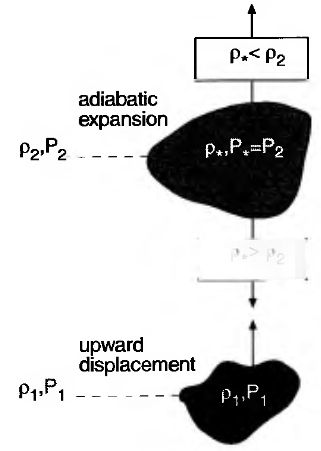
\includegraphics[width=3.5cm]{figures/convective_blobs.png}
\caption*{Source: Prialnik}
\end{figure}
\end{minipage}
%% Convection leads to \emph{circulation} of matter (but no net mass
%% transport).
}
%
%
\frame{
\frametitle{Schwarzschild criterion}
\begin{minipage}{0.4\linewidth}
\begin{itemize}
	\item Consider the atmospheres A, S, and S': the stably
          stratified case corresponds to S', where
          \begin{equation}
            \frac{\pd p}{\pd \rho} < \left(\frac{\pd p}{\pd \rho}\right)_{\rm a}\label{equ:Sch1}
          \end{equation}
        \item This form is not particularly useful so we will recast
          it in terms of a temperature gradient.
        \item Recall the 1st law of thermodynamics:
          \begin{equation}
            dQ = du + pdV.
          \end{equation}
\end{itemize}
\end{minipage}
\hfill
\begin{minipage}{0.59\linewidth}
\begin{figure}
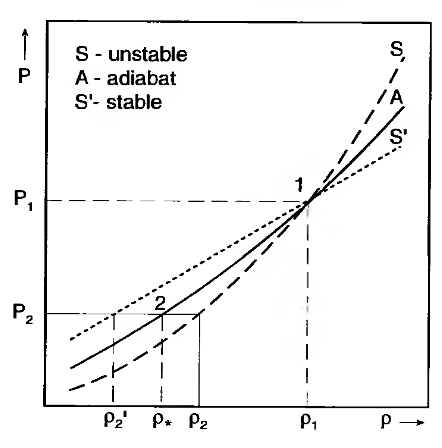
\includegraphics[width=6cm]{figures/pvsrho_convection.png}
\caption*{Source: Prialnik}
\end{figure}
\end{minipage}
}
%
\frame{
\frametitle{Schwarzschild criterion}

\begin{itemize}
\item The ideal gas equation can be written as:
  \begin{equation}
    p = {\cal R}_{\rm spec} \rho T = (c_p - c_V) \rho T,
  \end{equation}
  where $c_p = \left.\frac{dQ}{dT}\right|_{p}$ and $c_V =
  \left.\frac{dQ}{dT}\right|_V$ are specific heat capacities at
  constant pressure and at constant volume (unit
  J~K$^{-1}$~kg$^{-1}$). Their ratio is $\gamma = c_p/c_V = 5/3$ (aka
  adiabatic index).
\item Furthermore, with the specific internal energy $u = c_V T$ this
  becomes
  \begin{equation}
    p = {\cal R}_{\rm spec} \rho T = (\gamma - 1) \rho u,\ \ \mbox{and} \ \ u = \frac{1}{\gamma-1} \frac{p}{\rho}. 
  \end{equation}
\end{itemize}
}
%
\frame{
\frametitle{Schwarzschild criterion}

\begin{itemize}
\item For an adiabatic process $dQ = 0$. Furthermore, the specific
  volume is $V = \rho^{-1}$, and $dV = -d\rho/\rho^2$. Thus,
  \begin{equation}
    \frac{1}{\gamma-1} \left(\frac{dp}{\rho} - p \frac{d\rho}{\rho^2} \right) - p \frac{d\rho}{\rho^2} = 0.
  \end{equation}
  \begin{equation}
    \frac{1}{\gamma-1} \left(\frac{dp}{p} - \frac{d\rho}{\rho} \right) - \frac{d\rho}{\rho} = 0.
  \end{equation}
  \begin{equation}
    \frac{1}{\gamma-1} \left(\frac{\rho}{p}\frac{dp}{d\rho} - 1 \right) - 1 = 0.
  \end{equation}
  \begin{equation}
    \frac{\rho}{p}\frac{dp}{d\rho} = \left(\frac{\rho}{p}\frac{dp}{d\rho}\right)_{\rm a} = 1 + (\gamma - 1) = \gamma.
  \end{equation}
\end{itemize}
}
%
\frame{
\frametitle{Schwarzschild criterion}

\begin{itemize}
\item Going back to Eq.~(\ref{equ:Sch1}) we can write:
  \begin{equation}
    \frac{\rho}{p}\frac{dp}{d\rho} < \left(\frac{\rho}{p}\frac{dp}{d\rho}\right)_{\rm a} = \gamma.\label{equ:adia1}
  \end{equation}
\item For an ideal gas
  \begin{equation}
    \frac{dp}{p} = \frac{d\rho}{\rho} + \frac{dT}{T}.
  \end{equation}
\item Multiply by $p/dp$, make use of Eq.~(\ref{equ:adia1}) and define
  $\nabla_{\rm a}$:
  \begin{equation}
    1 = \left(\frac{p}{\rho}\frac{d\rho}{dp} + \frac{p}{T} \frac{dT}{dp}\right)_{\rm a} \equiv \frac{1}{\gamma} + \nabla_{\rm a},
  \end{equation}
  or:
  \begin{equation}
    \nabla_{\rm a} = 1 - \frac{1}{\gamma} = \frac{\gamma-1}{\gamma}.
  \end{equation}
\end{itemize}
}
\frame{
\frametitle{Schwarzschild criterion}

\begin{itemize}
\item Extending the definition of $\nabla$ to the general case 
  \begin{equation}
    \nabla \equiv \frac{p}{T}\frac{dT}{dp},
  \end{equation}
  we can rewrite the stability condition (\ref{equ:adia1}) as
  \begin{equation}
    \nabla < \nabla_{\rm a}.
  \end{equation}
  This criterion was derived by Karl Schwarzschild in 1906.
\item Sometimes the quantity $\Delta\nabla = \nabla - \nabla_{\rm a}$
  (superadiabaticity) is used to denoted whether a layer is
  convectively stable or not.
\item In stellar convection zones (apart from the near-surface layers)
  $\Delta \nabla$ is very small, e.g., ${\cal O}(10^{-8}\ldots
  10^{-3})$ in the Sun.
\end{itemize}
}
%
\frame{
\frametitle{Schwarzschild criterion -- reflection}
\begin{itemize}
\item Violation of Schwarzschild criterion is a necessary but not
  sufficient condition for convection to occur (\blue{Why?})
\end{itemize}
}
%
\frame{
\frametitle{Schwarzschild criterion -- reflection}
\begin{itemize}
\item Violation of Schwarzschild criterion is a necessary but not
  sufficient condition for convection to occur (\blue{Why?})
\item Internal friction in the gas was been neglected $\rightarrow$ in
  reality $\Delta \nabla$ has to exceed a finite value $\Delta
  \nabla_{\rm min}$ (which depends on $T$, $\rho$, rotation, magnetic
  fields, etc.) for convection to ensue.
\item Typically this is represented by a Rayleigh number which is a
  ratio of convective transport to diffusive transport:
  \begin{equation}
    {\rm Ra} = \frac{g d^4}{\nu\chi H_p} \Delta\nabla,
  \end{equation}
  where $g = GM/r^2$, $\nu$ is the kinematic viscosity, $\chi = K_{\rm
    rad}/\rho c_p$ is the radiative diffusivity, and $H_p$ is the
  pressure scale height.
\item Critical value for free convection is ${\rm Ra}_{\rm c} \approx
  1707$. In the Sun, ${\rm Ra} \approx 10^{20}$.
\end{itemize}
}
%
\frame{
\frametitle{When and why does convection happen?}

The Schwarzschild criterion is very general and we would like to have
something more spectific to stars.
\begin{itemize}
\item Consider a radiative star in hydrostatic equilibrium where the
  whole luminosity is transported by radiative diffusion:
  \begin{equation}
    F = - 4\pi r^2 K \frac{\pd T}{\pd r},
  \end{equation}
  where $K$ is the radiative conductivity:
  \begin{equation}
    K = \frac{16\sigma T^3}{3\kappa \rho} = \frac{4 c T^3}{3 a \kappa \rho}.
  \end{equation}
\item With this the temperature gradient is
  \begin{equation}
    \frac{\pd T}{\pd r} = - \frac{3}{4ac} \frac{\kappa \rho}{T^3} \frac{F}{4\pi r^2}.\label{equ:dTdr}
  \end{equation}
\end{itemize}
}
%
\frame{
\frametitle{When and why does convection happen?}

\begin{itemize}
\item Recast this in terms of radiative pressure:
  \begin{equation}
    \prad = \onethird a T^4, \ \ \mbox{or}\ \ d\prad = \fourthirds T^3 dT.
  \end{equation}
\item Now we can write the equation in terms of $\prad$:
  \begin{equation}
    \frac{d\prad}{dr} = - \kappa \rho \frac{F}{4\pi r^2}.
  \end{equation}
\item Finally, we use the hydrostatic equation:
  \begin{equation}
    \frac{dp}{dr} = - \rho \frac{Gm}{r^2},
  \end{equation}
  to obtain:
  \begin{equation}
    \frac{d\prad}{dp} = \frac{\kappa F}{4\pi Gm}.
  \end{equation} 
\end{itemize}
}
%
%
\frame{
\frametitle{When and why does convection happen?}

\begin{itemize}
\item The sought relation is:
  \begin{equation}
    \frac{d\prad}{dp} = \frac{\kappa F}{4\pi Gm}.
  \end{equation} 
\item \blue{What can you say based on this equation?}
\end{itemize}
}
%
%
\frame{
\frametitle{When and why does convection happen?}

\begin{itemize}
\item The sought relation is:
  \begin{equation}
    \frac{d\prad}{dp} = \frac{\kappa F}{4\pi Gm}.
  \end{equation} 
\item \blue{What can you say based on this equation?}
\item Because $p = \pgas + \prad$, $dp > d\prad$, or
  $\frac{d\prad}{dp} < 1$.
\item This means that for a \emph{radiative} star
  \begin{equation}
    \kappa F < 4\pi Gm.\label{equ:EddF}
  \end{equation}
\item This condition can be violated, and part of the energy must be
  transported by means other than radiation, if $\kappa F$ is
  sufficiently big.
\item Increase $\kappa$ due to partial ionization: outer layers of low
  mass stars such as the Sun.
\item Increase $F$ due to strong temperature dependence of energy
  production: CNO-cycle and triple-$\alpha$ in massive stars.
\end{itemize}
}
%
%
\frame{
\frametitle{Eddington luminosity}

\begin{itemize}
\item Eq.~(\ref{equ:EddF}) can be rewritten in terms of $L$ and $M$
  \begin{equation}
    L < \frac{4\pi G M}{\kappa}.
  \end{equation}
\item This is a fundamental limit for radiative luminosity (Eddington
  luminosity). If $L$ exceeds this, a radiation-driven \emph{stellar
  wind} will commence.
\end{itemize}
}
%
%
\frame{
\frametitle{Energy transport revisited}

\begin{itemize}
\item For a radiative star the total flow of energy (unit: W) is
  transported by radiation and given by
  \begin{equation}
      F = \Frad = 4\pi r^2 \frac{4ac}{3} \frac{T^4}{\kappa \rho H_p} \nabla_{\rm rad},
  \end{equation}
  where $\nabla_{\rm rad}$ is the radiative temperature gradient; see,
  Eq.~(\ref{equ:dTdr}).
\item When convection is present $F = \Frad + \Fconv \neq \Frad$, and
  therefore $\nabla \neq \nabla_{\rm rad}$.
\item Therefore we need to compute $\Fconv$ in order to calculate
  $\nabla$.
\end{itemize}
}
%
%
\frame{
\frametitle{Mixing length theory}

Convection is highly turbulent and chaotic, and occurs in 3D. This in
itself is already a nearly unsolvable problem (next lecture). Stellar
evolution models require a simple presciption of convection in 1D
(although there is no rigorous way to do this!).
\begin{itemize}
\item Assume discrete gas elements that move a vertical distance
  $\ell$ before dissolving.
\item This distance is called the \emph{mixing length}, and is given
  by $\ell = \aMLT \Hp$, where $\aMLT = {\cal O}(1)$. The functional
  form is a choice and cannot be derived rigorously from first
  principles!
\item The mixing length theory is analogous to the concept of
  mean-free path in thermodynamics. It originates from Ludwig Prandtl
  (1925) who used it to describe turbulent motions in the laboratory.
\item It was adapted to astrophysics by Ludwig Biermann in the 1930s
  and the most widely used version is due to Erika Vitense (1953); see
  also B\"ohm-Vitense (1958).
\item \blue{What can you conclude from the basic assumption of the
  mixing length theory?}
\end{itemize}
}
%
\frame{
\frametitle{Mixing length theory}

Pressure scale height increases with depth $\rightarrow$ convection
cells get bigger.

\begin{figure}
  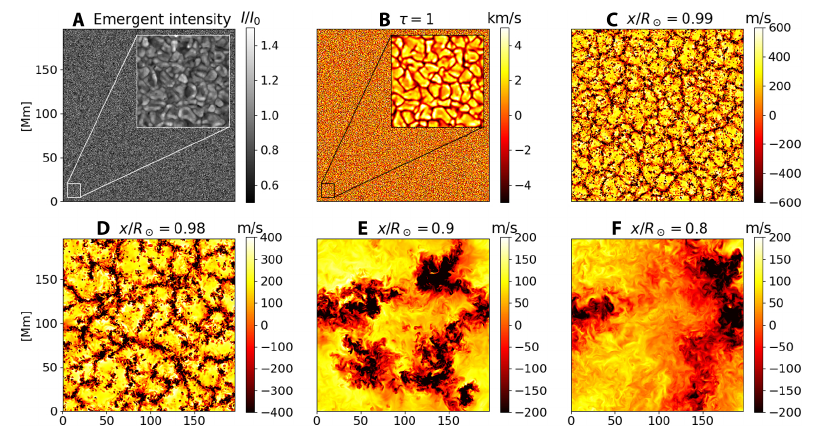
\includegraphics[width=10cm]{figures/Hotta_2019.png}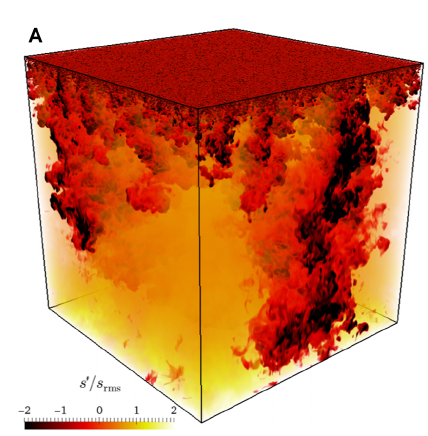
\includegraphics[width=5cm]{figures/Hotta_2019_box.png}
\caption*{Source: Hotta et al. (2019), \emph{Science Advances}, 5, 2307}
\end{figure}
}
%
\frame{
\frametitle{Mixing length theory}

\begin{itemize}
\item Consider the convective energy (more precisely enthalpy) flux
  (unit: W/m$^2$) is:
  \begin{equation}
    \Fconv = c_p \rho u \delta T,\label{equ:Fconv}
  \end{equation}
  where $u$ is the convective velocity, and $\delta T = T -
  \overline{T}$.
\item Assume that the ``average'' convective blob has traveled a
  distance $d=\ell/2$.
\item Then the temperature fluctuation is:
  \begin{eqnarray}
    \frac{\delta T}{T} = \frac{d}{T}\left(\frac{\pd T}{\pd r} - \left.\frac{\pd T}{\pd r} \right|_{\rm ad} \right) = (\nabla - \nabla_{\rm ad}) \frac{\ell}{2 H_p}, \label{equ:deltaT}
  \end{eqnarray}
\item Assume that half of the work done by the buoyancy force when
  travelling a radial distance $\ell/2$ goes to kinetic energy:
  \begin{eqnarray}
    - \frac{1}{2} g \frac{\delta \rho}{\rho} \frac{\ell}{2} = \frac{1}{2} g \frac{\delta T}{T} \frac{\ell}{2} = (\nabla - \nabla_{\rm ad}) \frac{g\ell^2}{8 H_p}.
  \end{eqnarray}
\end{itemize}
}
%
%
\frame{
\frametitle{Mixing length theory}

\begin{itemize}
\item Assume that half of this goes to the kinetic energy of the fluid element:
  \begin{eqnarray}
    u^2 = (\nabla - \nabla_{\rm ad}) \frac{g\ell^2}{8 H_p}.\label{equ:u2}
  \end{eqnarray}
\item Combining Eqs.~(\ref{equ:deltaT}) and (\ref{equ:u2}) gives the
  convective flux:
  \begin{equation}
    \Fconv = c_p \rho T g^{1/2} \frac{\ell^2}{4\sqrt{2}H_p^{3/2}} (\nabla-\nabla_{\rm ad})^{3/2}.
  \end{equation}
  \item \blue{What do these equations imply? Hint: recall the Schwarzschild criterion.}
  \item \blue{We made a shortcut in the analysis here. Any idea what this was?}
\end{itemize}
}
%
\frame{
\frametitle{Mixing length theory}

\begin{itemize}
  \item \blue{What do these equations imply? Hint: recall the
    Schwarzschild criterion.}
  \item The factor $\nabla-\nabla_{\rm ad}$ means that when the
    stratification changes from unstable to stable the convective flow
    abruptly stops. Therefore mixing length theory is \emph{local} and
    does not allow \emph{overshooting}.
  \item \blue{We made a shortcut in the analysis here. Any idea what
    this was?}
  \item There are still radiative losses from the convective fluid
    elements and therefore the temperature gradient inside the element
    ($\nabla_{\rm e}$) is not equal to $\nabla_{\rm ad}$.
  \item This leads to an additional equation (known as the cubic
    equation) that needs to be solved for $\nabla$.
  \item However, this is only important very near the surfaces of
    stars and many stellar evolution codes simply set $\nabla =
    \nabla_{\rm ad}$ when the Schwarzschild criterion is violated.
\end{itemize}
}
%
%
\frame{
\frametitle{Mixing length theory}
\begin{minipage}{0.4\linewidth}
\begin{itemize}
\item Mixing length model of the solar convection zone.
\item Huge differences in pressure, density, superadiabaticity, and
  velocity.
\item Also the convective turnover time $\tau_{\rm c} = \ell/u$ varies
  several orders of magnitude.
\end{itemize}
\end{minipage}
\hfill
\begin{minipage}{0.4\linewidth}
\begin{figure}
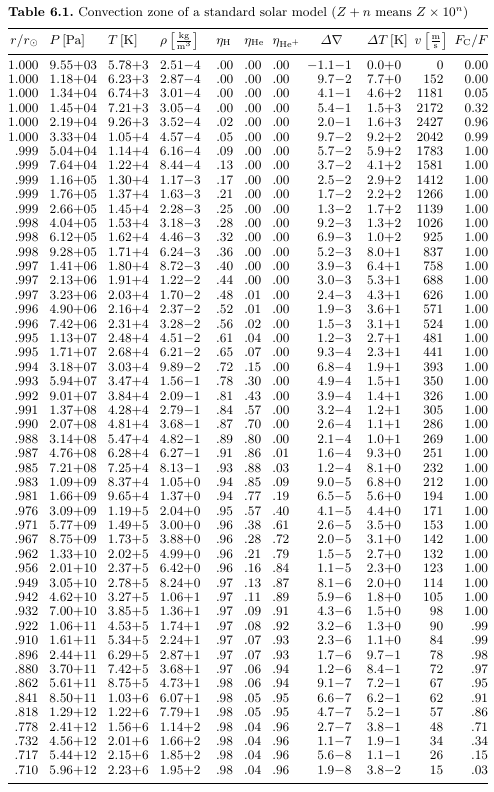
\includegraphics[width=4.75cm]{figures/MLT_Sun_Stix2002.png}
\caption*{Stix (2002), The Sun: An Introduction}
\end{figure}
\end{minipage}
}
%
%
\frame{
\frametitle{Mixing length theory vs. simulations}
\begin{minipage}{0.4\linewidth}
\begin{itemize}
\item Convective velocities in 3D simulations are of the same order of
  magnitude as from MLT.
\item Exact match cannot be expected beacuse MLT is a very coarse
  approximation + simulations have their own issues (next lecture).
\end{itemize}
\end{minipage}
\hfill
\begin{minipage}{0.5\linewidth}
\begin{figure}
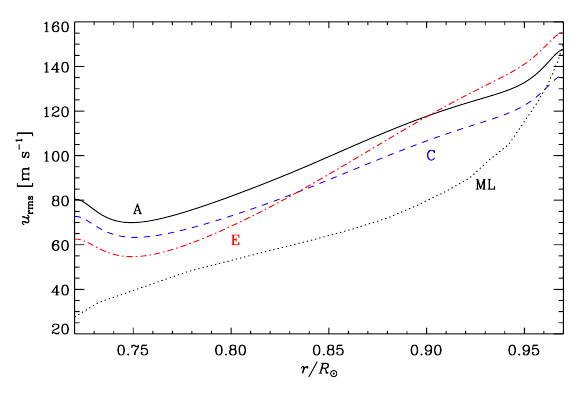
\includegraphics[width=8cm]{figures/uconv_KKB14.png}
\caption*{Average convective velocity in simulations (A, C, E) and
  from MLT}
\end{figure}
\end{minipage}
}
%
\frame{
\frametitle{Mixing length theory -- issues?}
\begin{itemize}
\item Non-rotating convection looks similar to what mixing length
  theory predicts.
\end{itemize}
\begin{figure}
  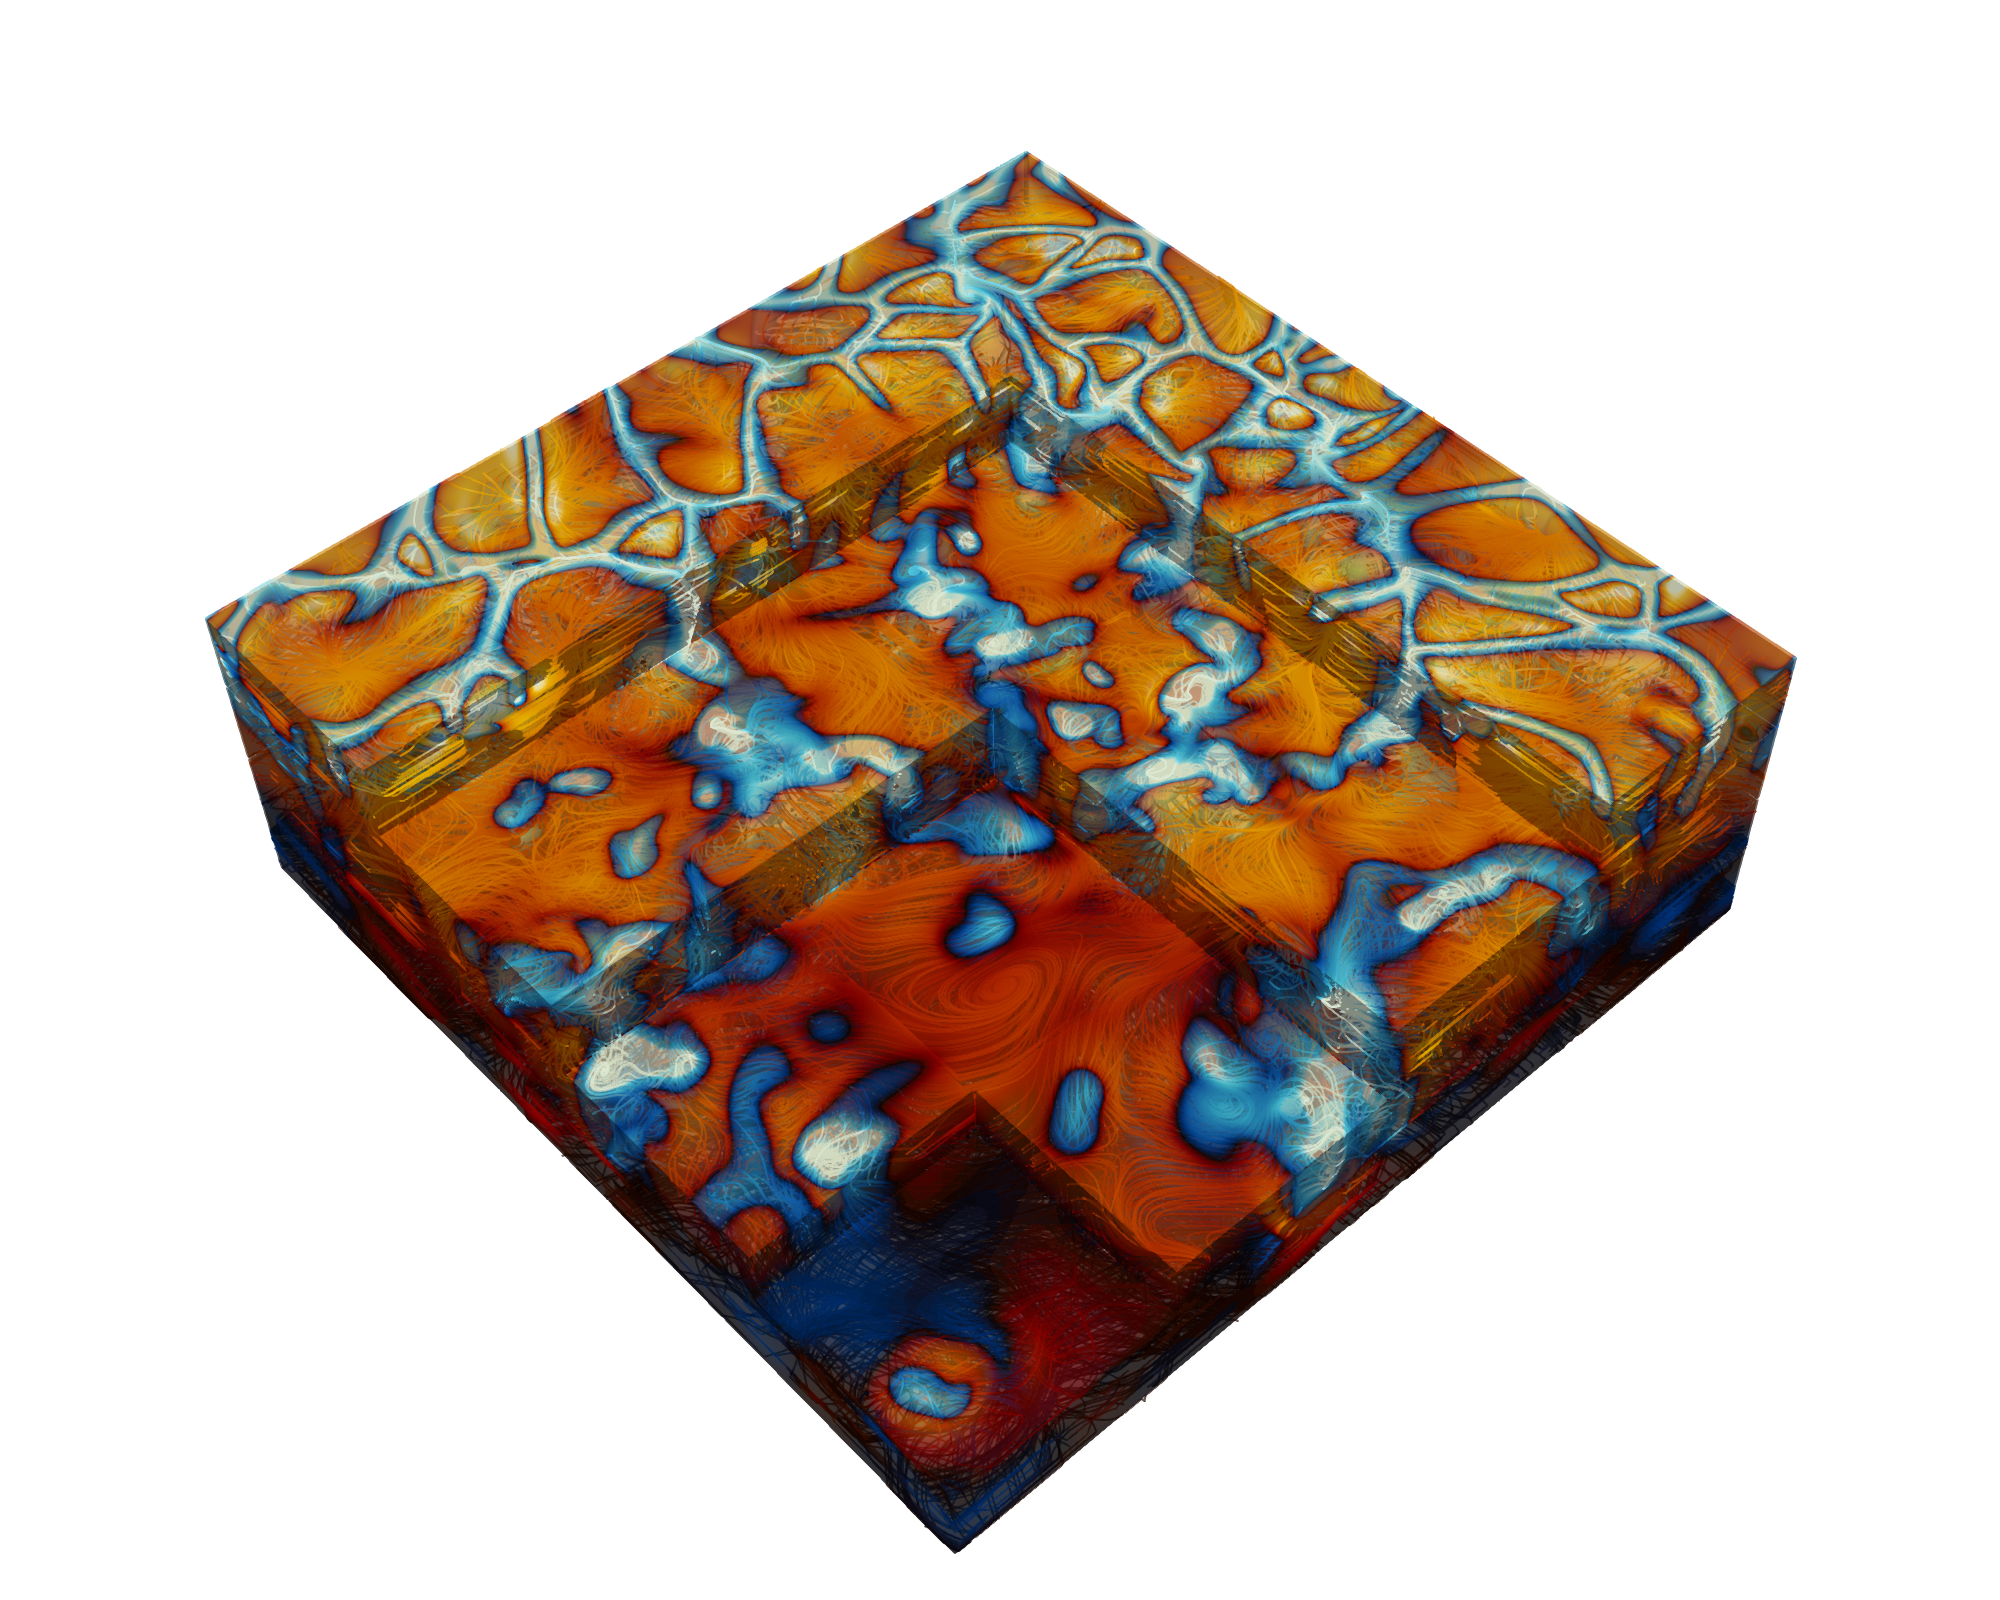
\includegraphics[width=7cm]{figures/conv-norot.png}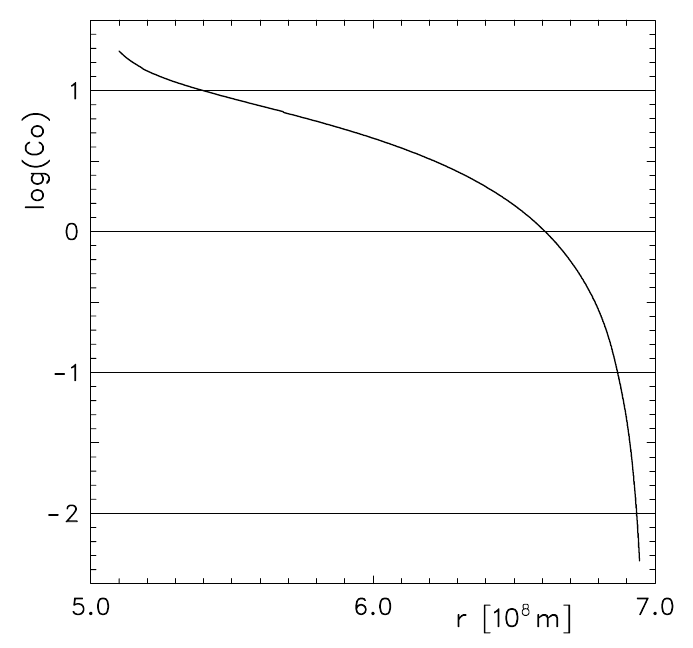
\includegraphics[width=6cm]{figures/MLT-Sun_Co.png}
\caption*{Left: Non-rotating convection. Right: logarithm of the
  Coriolis number ${\rm Co} = 2\Omega_\odot/\tau_{\rm c}$ using mixing
  length model data.}
\end{figure}
}
%
%
\frame{
\frametitle{Mixing length theory -- issues?}
\begin{itemize}
\item Non-rotating convection looks similar to what mixing length
  theory predicts. But not if rotation is sufficiently strong.
\end{itemize}
\begin{figure}
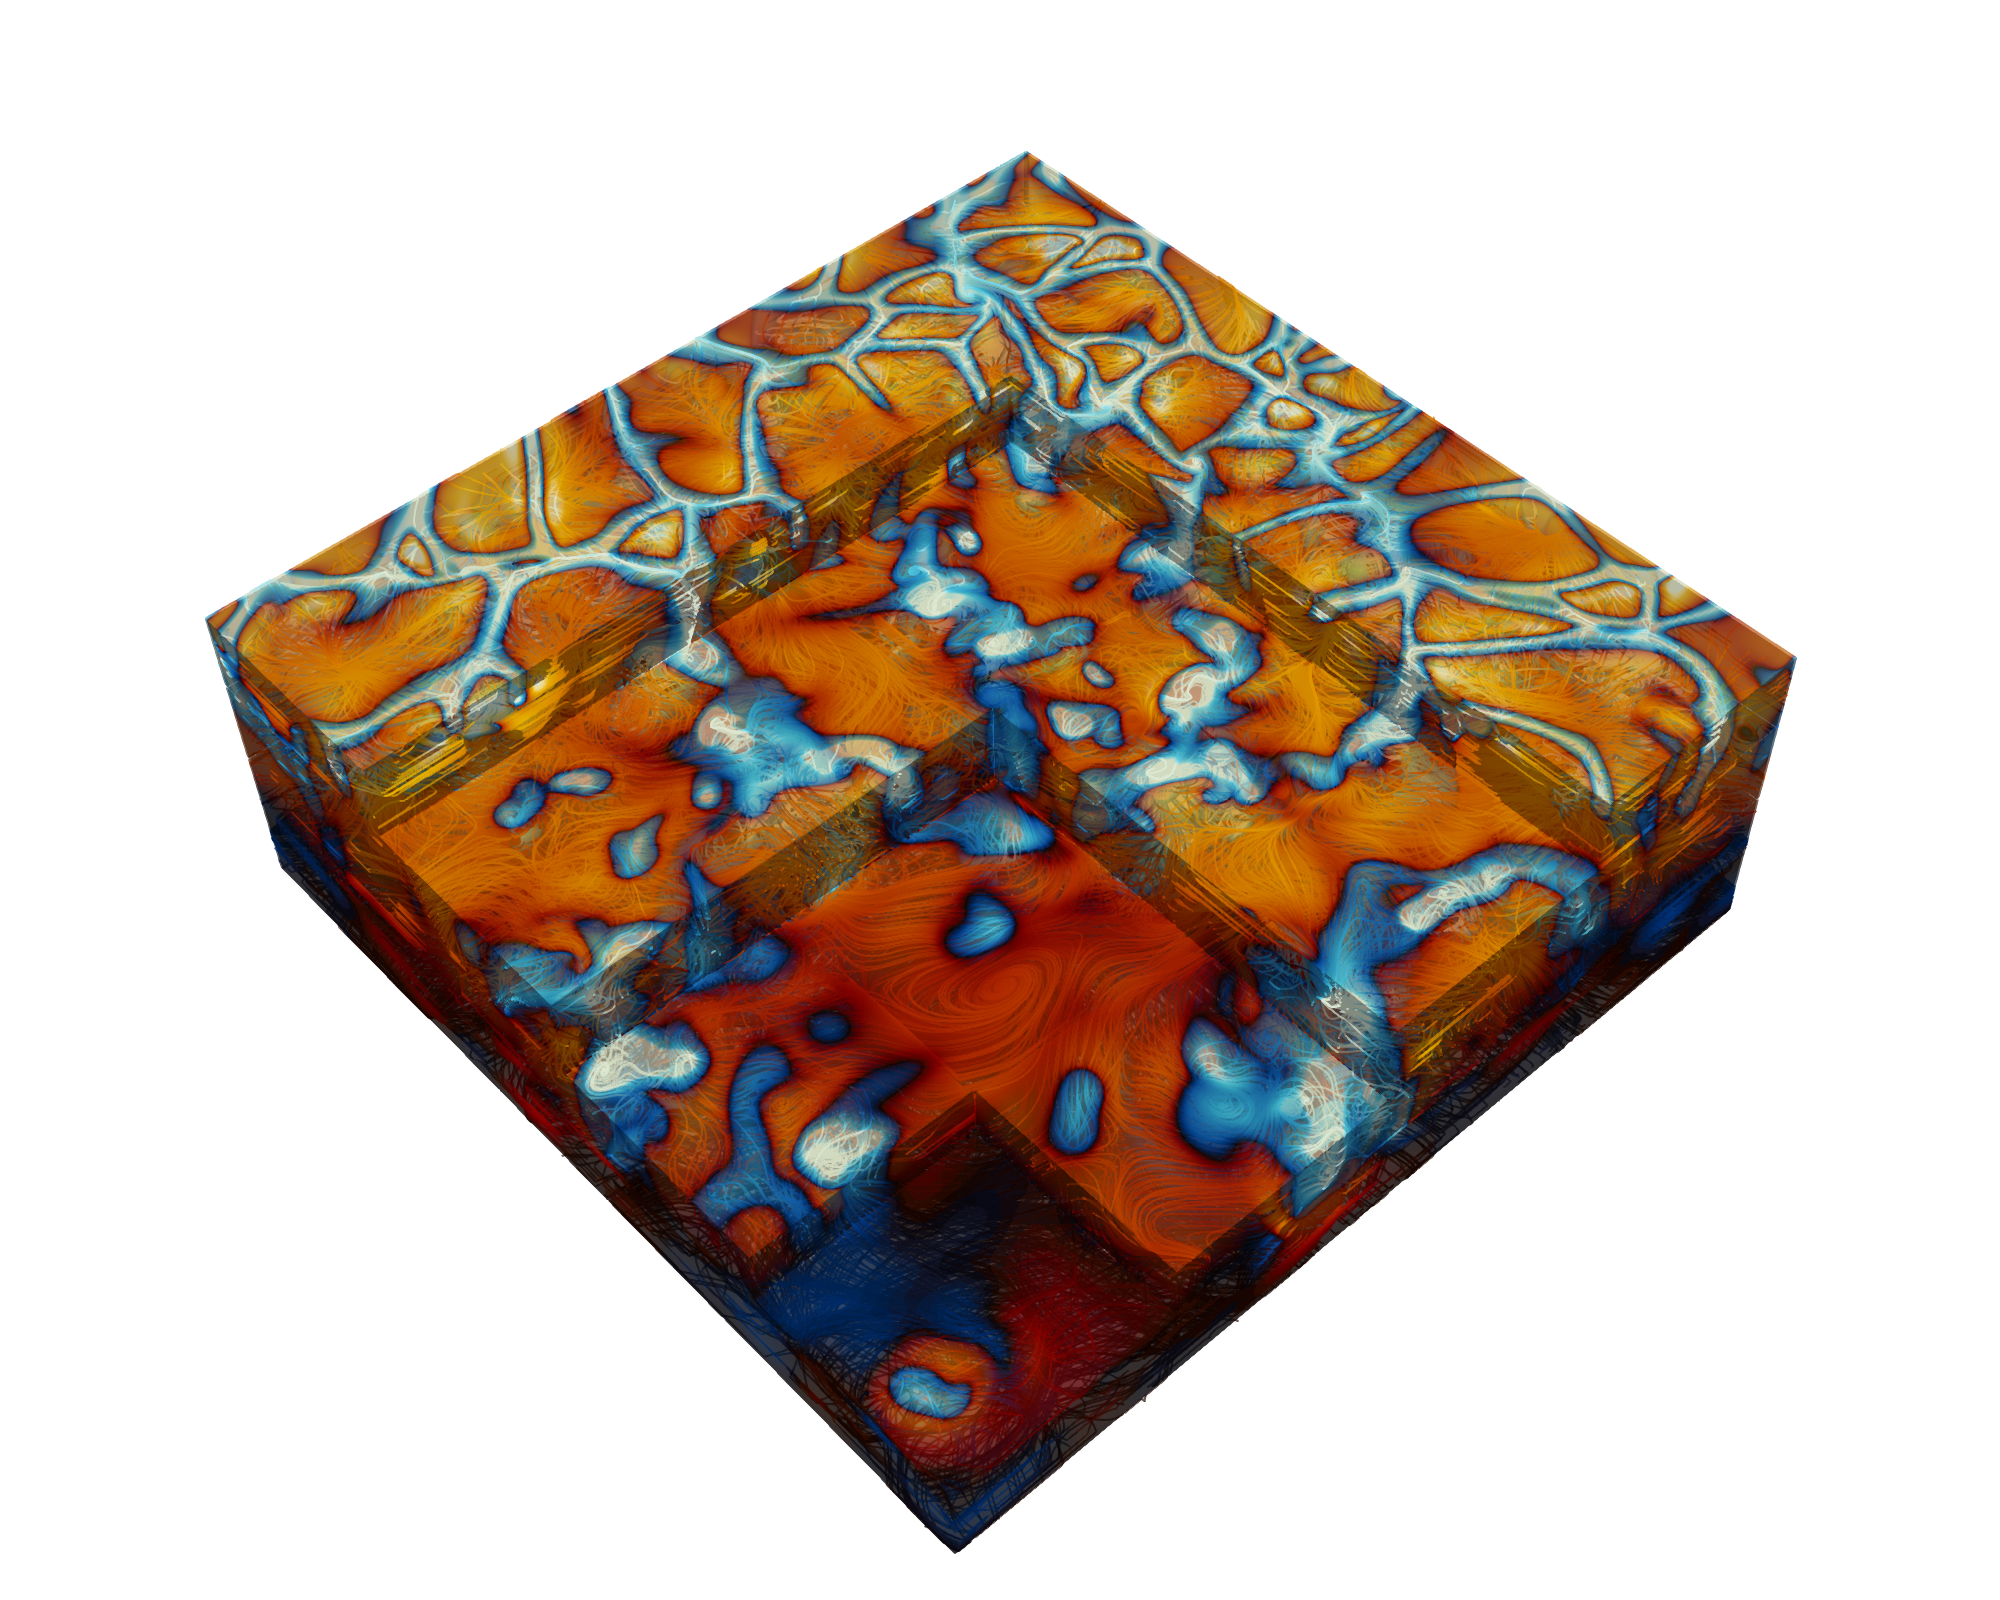
\includegraphics[width=7cm]{figures/conv-norot.png}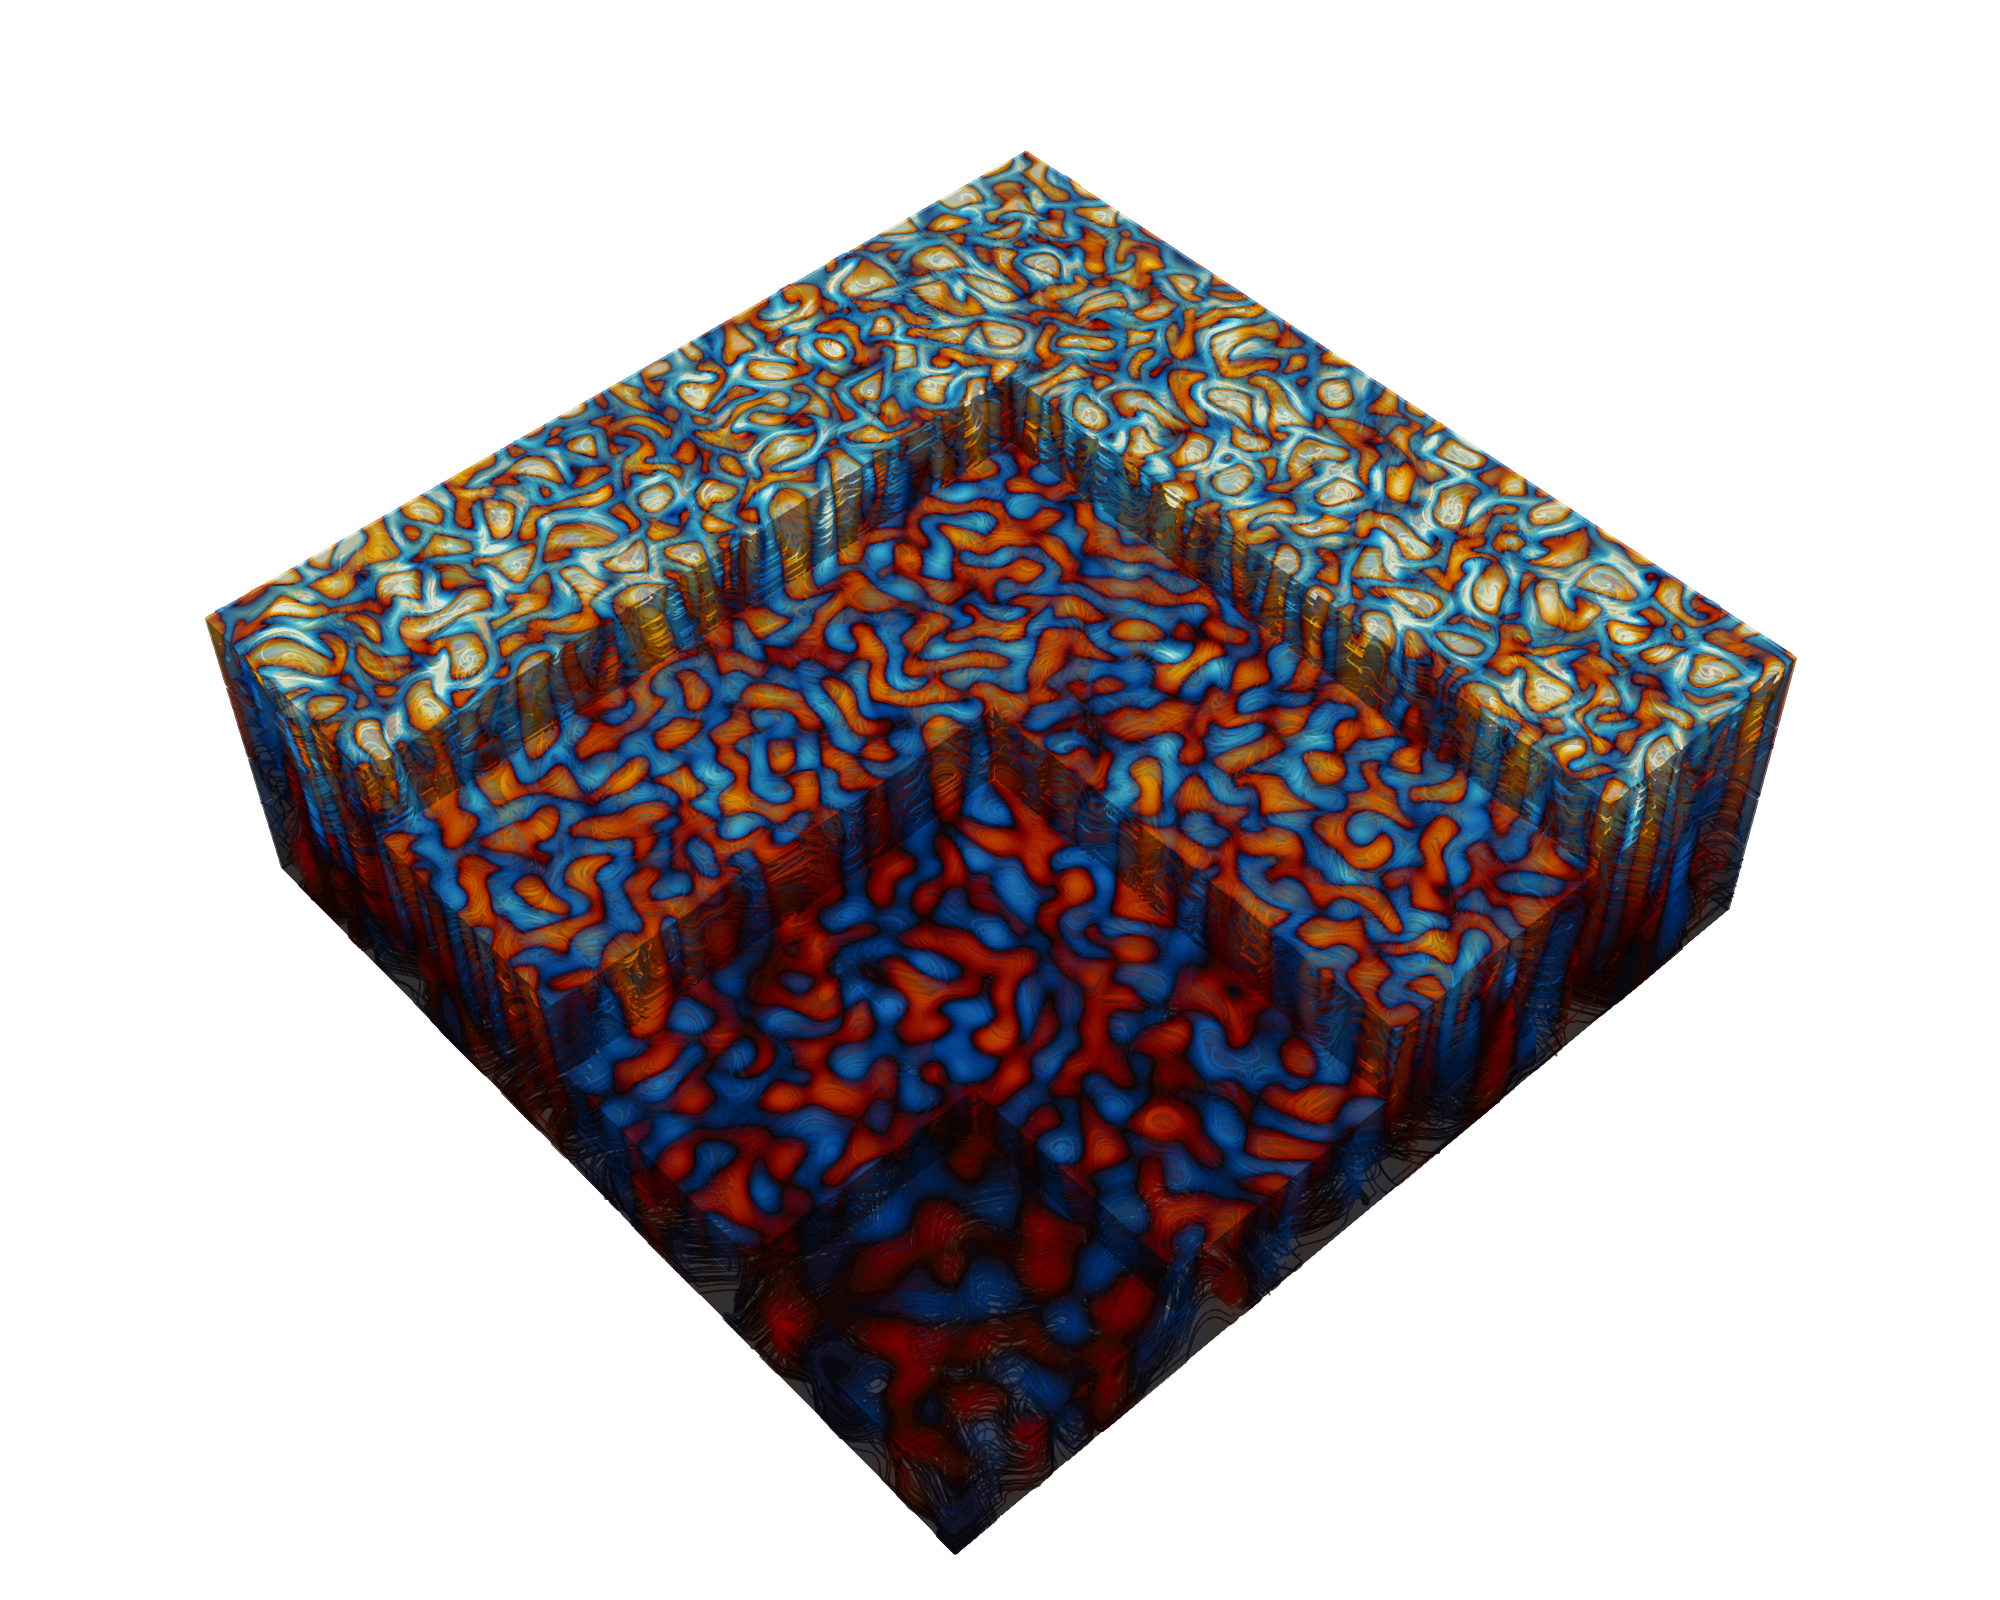
\includegraphics[width=7cm]{figures/conv-rapidrot.png}
\caption*{Left: Non-rotating convection. Right: rapidly rotating convection.}
\end{figure}
}
%
%
\frame{
\frametitle{Perfect is the worst enemy of good enough?}

\begin{itemize}
\item Mixing length theory (+ some additional tweaks to account for
  overshooting) is generally good enough to capture the big picture.
\item However, the interplay of convection, rotation and magnetism
  leads to another set of interesting problems that can also have
  repercussions to everyday life.
\end{itemize}
\
}

\end{document}



